%{\color{red}jh-change: 
% 10 03 2011 jh  fix format of f-line, commant about w_emap bug
% 25 04 2012 jh  add command fq

\subsection{HASH}
\index{HASH}
\label{HASH}

This program \citep{hardebeck2002,hardebeck2003} determines fault plane 
solutions using P-polarities and amplitude ratios as input, just like 
the FOCMEC program. The P-amplitude 
$A_P=\sqrt(A_r^2+A_z^2)$
 and the S-amplitude 
$A_S=\sqrt(A_{sv}^2+A_{sh}^2)$
 where A 
is amplitude, r is radial, z is vertical, sv is SV, and sh is SH. 
The free surface correction is not built in, but replaced by a fixed 
factor per station, which has to be determined independently. In order 
to simplify the input, the free surface corrected amplitude ratios 
from FOCMEC are used as input for HASH. The program was modified 
to use only SH and by using the free surface corrected P on the Z-component, 
the assumption is made that $A_p = A_z(P)$. Thus only one amplitude 
ratio is used for each station (SH to P). HASH returns solutions with 
less than a given number of polarity errors and average amplitude 
errors less than a given limit. If no solutions are found, error limits 
are increased and normally many solutions are returned. Using this, 
an estimate of the best solution is made and likely errors calculated. 
The advantage with HASH is that it finds one or a few best solutions, 
while for FOCMEC the user must select one among many. Also HASH will 
not completely change the solution by one wrong amplitude ratio, since 
the average of the amplitude errors is used as selection criteria and 
not a single amplitude. FOCMEC does not give any estimate of the errors 
in the solution. HASH calculates an estimated error; however that requires 
an input where each event has been located with e.g. 10 different likely 
input models and all data is used as input in order to get estimate of 
fault plane solution uncertainties generated from the model. This was 
not done in the SEISAN implementation so only the error estimated from 
the spread in solutions is used.  This might lead to smaller error estimates 
as compared to the original HASH implementation. The SEISAN HASH implementation 
is a simplified implementation compared to the original HASH with many 
parameters hardwired, see hash\_seisan.for for implementation details and 
changes. Like FPFIT, the F-fit function is calculated (called weighted 
fraction of polarity misfits) and similarly the station distribution 
ratio (see FPFIT). Both values are given in S-file as well as the average 
amplitude error. For more information, see the HASH manual hash.pdf 
and FPFIT manual fpfit.pdf in INF. The software is found at 
\url{http://earthquake.usgs.gov/research/software/index.php}.
%http://earthquake.usgs.gov/research/software/index.php. 
HASH does 
not estimate errors in strike, dip and rake but errors in fault plane and auxiliary plane (degrees). 

Running HASH from EEV

Polarities and amplitudes are picked like for FOCMEC. When running the program, the amplitudes are corrected like for FOCMEC (actually done by FOCMEC) so the Q-correction will use the Q-relation given in focmec.def (see FOCMEC description above). The same output, as for FOCMEC, with the available amplitudes, their ratios and corrections will be shown and the control is the handed over to HASH. The questions are:

\begin{verbatim}
  Grid angle for focal mech. search, enter for def 2            Comment: Smallest is 2

  Max number of polarity errors                                 Comment: No default
1
  Max average error in amp rat, log10, def 0.2                  Comment: default 0.2 selected

  Enter angle for computing mechanisms probability, def is 60   Comment. Default 60 deg. Sel.

  Enter probability threshold for multiples, def is 0.1         Comment: Default 0.1 selected
\end{verbatim}

Now is following the FOCMEC amplitude information, not shown $\ldots$

\begin{verbatim}
 Number of polarities is                      :    11
 Number of amplitude ratios is                :     5
 Minimum number of polarity misfits overall   :     0     
 Minimum average amplitude error overall      :  0.13
 New number of pol. misfits inc. extra is     :     1
 New average amp limit inc. extra             :  0.23
 Minimum average amplitude error for pol ok   :  0.27
 New average amp limit is                     :  0.37
 Number of solutions found                         92

 Strike,dip,rake               197.3    66.5  -157.4
 Fault+aux plane uncertainty    23.2    10.3
 ================================
\end{verbatim}

Explanations on input:

The "mechanism probability" is the probability that the real mechanism 
is "close" to the preferred mechanism, within "angle for computing 
mechanisms probability" where angle define "close." If there are 
clustered outliers, alternative solutions (or "multiples") are found 
based on those outliers. You can set the minimum probability for the 
multiples (i.e. ignore multiples with a low probability.)

Explanations on output:

\verb|Minimum number of polarity misfits overall|: 
Minimum number of wrong polarities for anyone of the grid points 
disregarding amplitude fit. This is the number of polarity errors 
to find a solution without amplitudes.   \newline
\verb|Minimum average amplitude error overall|: The minimum average log error for any grid point disregarding errors in polarity.\newline
\verb|New number of pol. misfits inc. extra is|: The new limit for polarity errors.     \newline
\verb|New average amp limit inc. extra|: Based on the above, a new amplitude ratio error limit is set.\newline
\verb|Minimum average amplitude error for pol ok|: The new error limit considering polarities within limit.\newline
\verb|New average amp limit is|: In order to get sufficient solutions, the amplitude error limit is increased to this value.\newline
             
Output files:
Hash\_seisan.out: A summary of the solutions(s).\newline
Fps.out: The solution(s) in SEISAN format.

\textbf{Storing and selecting fault plane solutions: Format errors estimates and quality.}

The fault plane solutions are stored in the S-file. Different programs give somewhat 
different parameters and sometimes the same output field is used for 
different parameters. Some programs give strike of dip instead of 
strike of fault plane, but values used in SEISAN are converted to 
strike of fault plane. Each program is indicated with its own name 
like "\verb|HASH     F|" at the end of the F-line. If no characters are 
written in the blank space, any new solution will overwrite the old 
one. However if anything is written like "\verb|HASH    1F|", any new solution 
will create a new line in S-file. This is also the case if a quality 
indicator is written (see below). An example is:

\begin{verbatim}
     158.0      53.1    -156.4  7.0  3.8      0.30 0.57 0.76      FCF HASH     F
   39.2900   66.3900  -63.6500                          0.13  2 1 FCF FOCMEC   F
      42.0      68.0     -62.0  7.0  5.0  3.0  0.1  0.2           FCF FPFIT  A F
      18.7      67.8     -63.3                                4   FCF PINV     F
\end{verbatim}

In this example, there are 4 solutions made by the 4 programs and the solution made by FPFIT has been selected as a prime solution with quality A. The content and format is: 

\begin{verbatim}
Type F Line (Optional): Fault plane solution 

Columns Format Description

  1:30 3F10.0 Strike, dip and rake, Aki convention
 31:45 4F5.1  Error in strike dip and rake (HASH), error in fault plane and aux. plane (FPFIT) 
 46:50 F5.1   Fit error:  FPFIT and HASH (F-fit)
 51:55 F5.1   Station distribution ratio (FPFIT, HASH)
 56:60 F5.1   Amplitude ratio fit (HASH, FOCMEC)
 61:62 I2     Number of bad polarities (FOCMEC, PINV) 
 64.65 I2     Number of bad amplitude  ratios (FOCMEC)
 67:69 A3     Agency code
 71:77 A7     Program used
 78:78 A1     Quality of solution, A (best), B C or D (worst), added manually
 79:79 A1     Blank, can be used by user
 80:80 A1     F
\end{verbatim}


\verb|Quality indicator|: The indicator can be any character, but usually A to F is used with A as the best. It is up to the user to manually assign a quality indicator. Events can later be selected based on quality indicator. Programs SELECT and FOC use quality indicators. The quality indicator as well as the selection of the prime solution can be select by command fq in eev. An example is given below:

% jh change, following should be courier, smaller font

  Fault plane solutions for this event
 1  180.3      55.1    -123.7  5.0  4.4      0.04 0.67 0.38      SJA HASH   A
 2 6.1000   48.4400  -48.0700                               2    SJA FOCMEC
 3  191.0      51.0    -110.0                                    SJA DREGER
 4  185.0      48.0    -121.0                                    HRV CMT    A
  Give fps number to be prime solution, enter for no change




\textbf{Composite fault plane solutions}

A composite solutions means that data from several events, suspected to have the same fps, will be used together. Composite solutions can be useful if little data is available. All programs except INVRAD can be used for a composite solution. Composite solutions must be calculated outside EEV and the solutions therefore do not become part of the data base. Both amplitudes and polarities can be used. Local and global data can be used. The procedure is:

\begin{itemize}
\item Select events to be used together in one cat file, e.g. by using SELECT.
\item
Locate the events with HYP, there will then be a hyp.out and a print.out, which are used as input for the composite solution.
\item Start one of the 4 fps programs: FOCMEC, PINV, FPFIT\_SEISAN or HASH\_SEISAN. The usual questions will come up. 
\item The solution(s) will be written in the individual program output file. The solution(s) will also be written to the cat-file fps.out in standard SEISAN format. For each run of a program, the solutions accumulate in fps.out. This can be used to compare solutions from different programs, see FOC. An example of the plot is seen in Figure \ref{fig:foc}. To plot the observations, put in solution
in hyp.out and plot with FOCMEC.
\end{itemize}
 
\begin{figure}
\htmlimage{scale=2.0}
\centerline{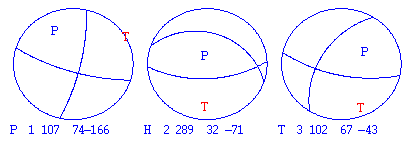
\includegraphics[width=0.9\linewidth]{fig/foc}}
\caption{Using FOC to plot solutions from fps.out. The program used 
for each solution is given with a one letter code: P: PINV, F: FOCMEC, H: HASH and T: FPFIT.}
\label{fig:foc}
\end{figure}


\textbf{Which program to use}

The different programs all have advantages and disadvantages. FOCMEC uses the most data since it can use more amplitude ratios than HASH but it might be difficult to find the 'correct' solution since a small change in input limits might make a large change in output. If a few of the amplitude ratios are very wrong, an unrealistic high ratio limit must be used and many errors allowed. This problem is avoided by using HASH since the limit is the average amplitude ratio error and not the number of errors. If only working with polarities, all 4 programs can be used. PINV gives a very quick solution which can be used as an indication of a possible best solution, however for final results one of the other 3 programs should be used. It is often a good idea to compare the results from the different programs. Ideally they should all give the same result, but there will be difference due to different methods used and different data, however if solutions are very different, the solution might not be very stable. It is easy to compare the solutions. Run each program in EEV, then plot using command fo. Each solutions will be plotted in a different color, see Figure \ref{fig:fps-compare}. If doing composite solutions, use program FOC with input from fps.out. 

\textbf{SLICK, inversion of fault plane solutions to get best stress tensor}

This program is part of the Slick package doing the following quoting the author \cite{michael1984} "The slick package uses fault slip data (either field observations or from focal mechanism) to find the stress tensor that best explains the observations. Inputs are the orientation and slip direction of a set of fault planes. Outputs are the orientation and shape of the stress ellipsoid, including confidence regions, and statistics used to judge the success of the inversion. This method uses the linear inversion algorithm and non-parametric bootstrap statistics". The software is available at 
\url{http://earthquake.usgs.gov/research/software/index.php}. 
%http://earthquake.usgs.gov/research/software/index.php. 

In SEISAN, only the inversion part has been implemented so the error analysis is missing. Program SLICK can be run as a separate program, but is normally run as part of FOC which prepares the input for SLICK and plots the output.  The method is explained in \cite{michael1984} where also examples are given with data available at the above web site.
Running SLICK: slick "file", where "file" is a file with strike of dip, dip and rake. An example input file is:

\begin{verbatim}
Strik dp     Dip    Rake
   203.0    51.0   137.0
   280.0    85.0  -161.0
    ...
\end{verbatim}

Note that in SEISAN, strike of fault plane is used so the strike of the dip is strike of the fault plane+90 degrees. The output is "file.oput" which gives the found stress tensor and the fit to the data, for details see \cite{michael1984}. The stress tensor has a corresponding slip angle, (average slip) and for each event the difference in slip angle for the individual event and the average slip is calculated as well as the average difference and standard deviation.  When running SLICK with FOC, an input file foc.slick is made for selected events (making the corrections to strike of slip) and the output file is foc.slick.oput. FOC also plots the direction of maximum compressive stress s1, minimum compress stress s3 and null axis s2. In the example below s1 has max value of 0.68 and strike and dip are 19 and 34 respectively. S3 has strike and dip of (113, 5) and s2 (-149, 56) respectively. The average fit angle is 59 with a standard deviation of 51, a bad fit.

\begin{verbatim}
stress tensor is:
-0.290526  0.236582  -0.146602  
0.236582  0.293028  -0.438347  
-0.146602  -0.438347  -0.00250278  
eigenvalue   vector: E,N,UP,direction,plunge
0.686771  -0.273399  -0.784281  0.556917  19.205739  33.820430
-0.37516  -0.917882  0.385856  0.0927811  112.725966  5.320093
-0.31161  0.287656  0.485818  0.82537  -149.270892  55.589101
variance= 0.283314
phi value= 0.940156

dip direction, dip, rake, fit angle, mag tau
  203.0     51.0    137.0    166.4    0.11
  280.0     85.0   -161.0    167.9    0.19
   ...
   13.9     68.1    -85.7     11.0    0.46
   14.0     70.0   -130.0     33.3    0.48
fit angle mean= 59.156784 standard deviation= 51.527176
for f=0.8 I= -2.242677 , std. dev.= 1.609795 D norm= 0.248640
avg tau=xx , std. dev.= xx
\end{verbatim}


For a complete stress analysis it is recommended to also do the error analysis using the complete slick package or e.g. the program ZMAP (not a SEISAN program, uses MATLAB, found at 
\url{http://www.earthquake.ethz.ch/software/zmap/ftp}).  
%http://www.earthquake.ethz.ch/software/zmap/ftp).  
FOC writes a file which is formatted for input to ZMAP. However doing stress analysis as implemented in SEISAN gives a good impression of the consistency of the fault plane solutions in a particular area. It is recommended that at least 10 events are used for inversion.
 

Plotting fault plane solutions

There a 4 ways of plotting fault plane solutions in SEISAN:  Through EEV (a single event), program FOC (many events), program EPIMAP (many events) and W\_EMAP (many events). The input file is in all cases a CAT-file. In addition, using program SEIGMT, a file to be used with GMT is prepared, however the use must make his own script. Only through EEV is it also possible to plot the observations.

Using EEV\newline
Command fo will plot all events in S-file. This can be a useful ways of comparing solutions obtained by different programs, see Figure \ref{fig:fps-compare}.

 

\begin{figure}
\htmlimage{scale=2.0}
\centerline{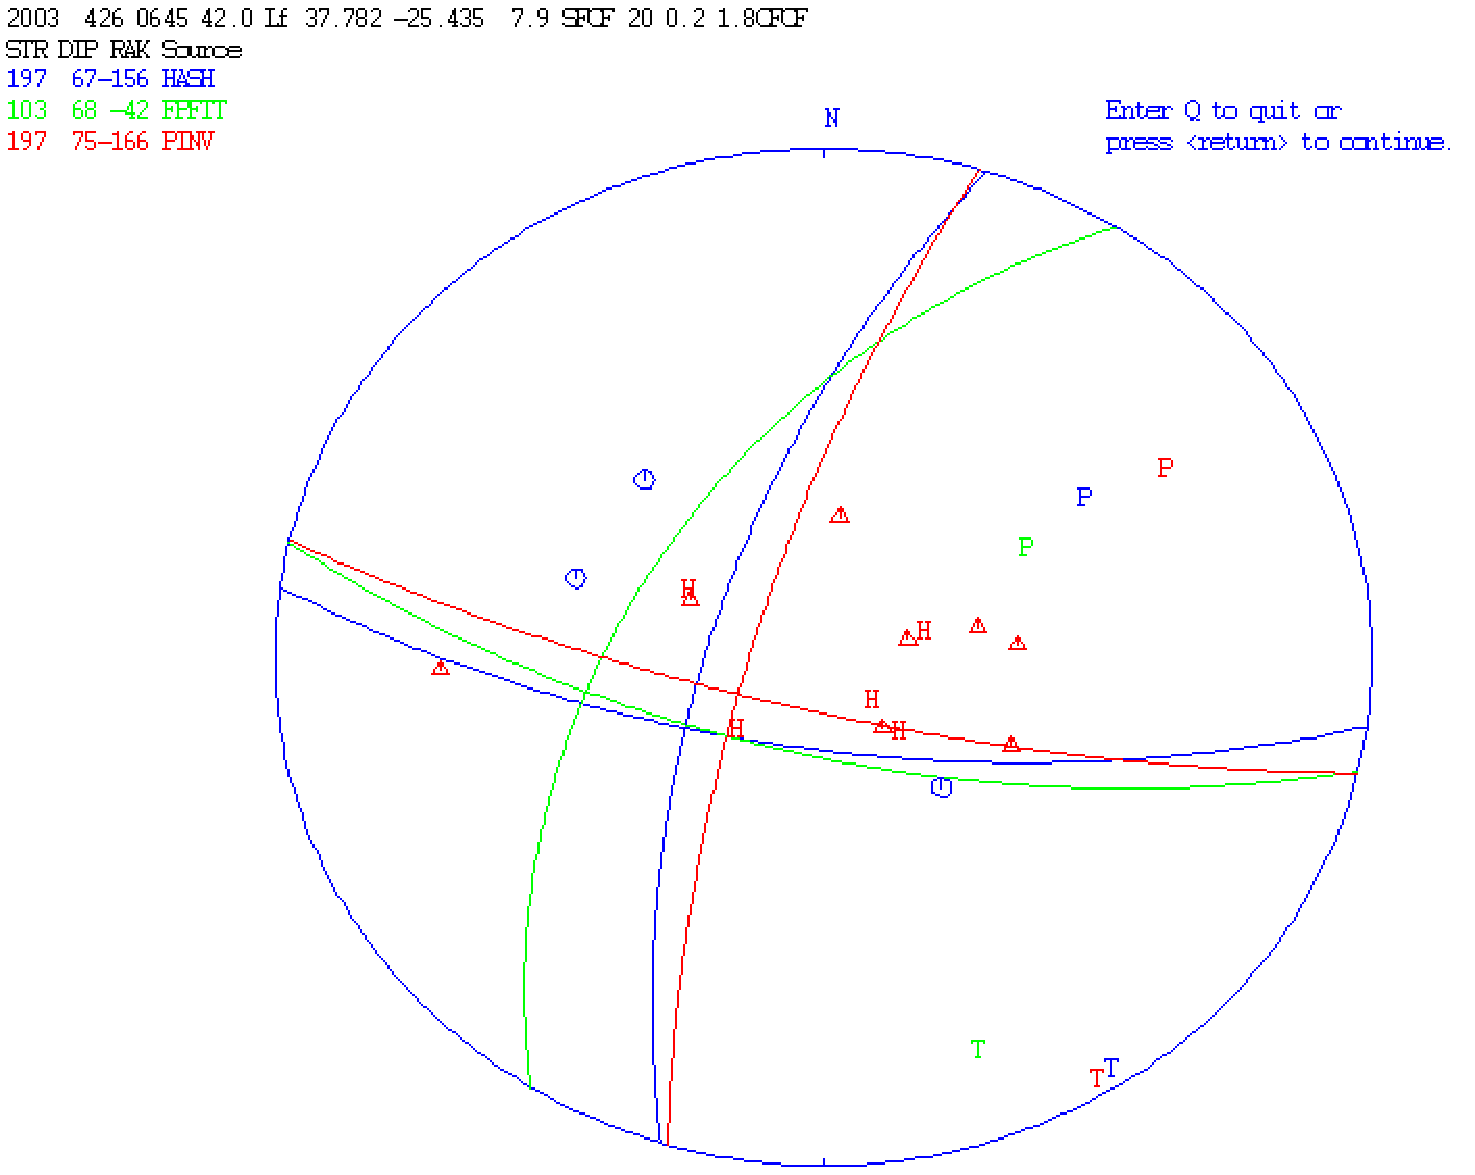
\includegraphics[width=0.9\linewidth]{fig/fps-compare}}
\caption{Compare fault plane solutions from different programs. For explanation of symbols, see FOCMEC.}
\label{fig:fps-compare}
\end{figure}


Using FOC\newline
See under FOC for how to run the program, see page
\pageref{page:foc}.
The plot is seen in Figure \ref{fig:foc}.


 
\begin{figure}
\htmlimage{scale=2.0}
\centerline{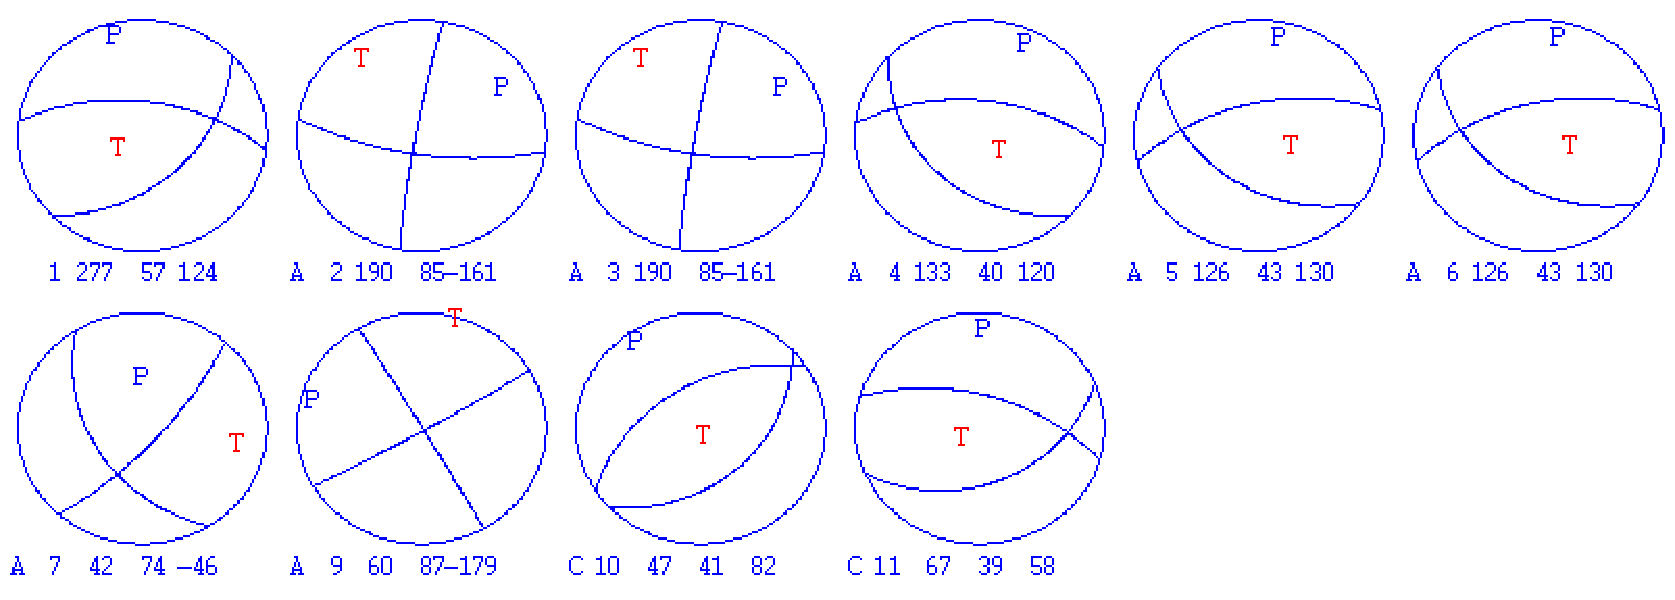
\includegraphics[width=0.9\linewidth]{fig/fps-many}}
\caption{Example of plotting many solutions. Each solution is given with number, the fault plane solution and the quality (A-E). Up to 24 solutions can be plotted on one page.}
\label{fig:fps-many}
\end{figure}


W\_EMAP (Windows only) plots the solutions as seen in Figure \ref{fig:fps-twomaps}. 
In this case the simplest is to give command w\_emap file, where file 
is the CAT file with fault plane solutions. See W\_emap manual in INF. 
NOTE: Some versions of W\_EMAP plots some of the fault plane solutions 
with inverted color e.g. inverse fault becomes a normal fault).

  

\begin{figure}
\htmlimage{scale=2.0}
\centerline{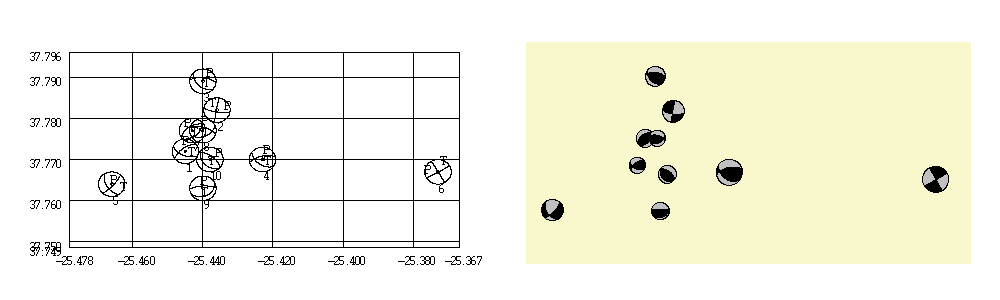
\includegraphics[width=0.9\linewidth]{fig/fps-twomaps}}
\caption{Plotting many fault plane solutions. Left: Using W\_EMAP. Notice that the colors in the solutions are inverted compared to normal practice. Right: Using EPIMAP. The data for the two plots is the same.}
\label{fig:fps-twomaps}
\end{figure}


The EPIMAP plot for the same events is shown in Figure \ref{fig:fps-twomaps}. See EPIMAP for more explanation. EPIMAP can also plot the fault plane solutions in a section, the solutions are still seen in the horizontal plane.


\textbf{FOC}
\label{page:foc}.

FOC is a program doing different things with fault plane solutions given in a CAT-file: Converting data to other formats, plotting many solutions, running the SLICK program and displaying the results, plot P and T axis for many events and make statistics of polarities. The input is:

\begin{verbatim}
foc
 Give input file
collect.out
 Quality, ABC.., up to 5 chars, enter for all
AB                                            Comment: Different qualities can be selected
 Cumulative(c) or individual misfit(def)      Comment: See later

 Plot all solutions selected (Y=enter/n)      Comment: Analysis can be done without plotting all
N
\end{verbatim}

The plot of the many fault plane solutions is seen in Figure \ref{fig:fps-slick}. 
After plotting the fault plane solutions, a plot comes up plotting 
the location of the P and T axis and the results from SLICK, see Figure \ref{fig:fps-slick}.

 
\begin{figure}
\htmlimage{scale=2.0}
\centerline{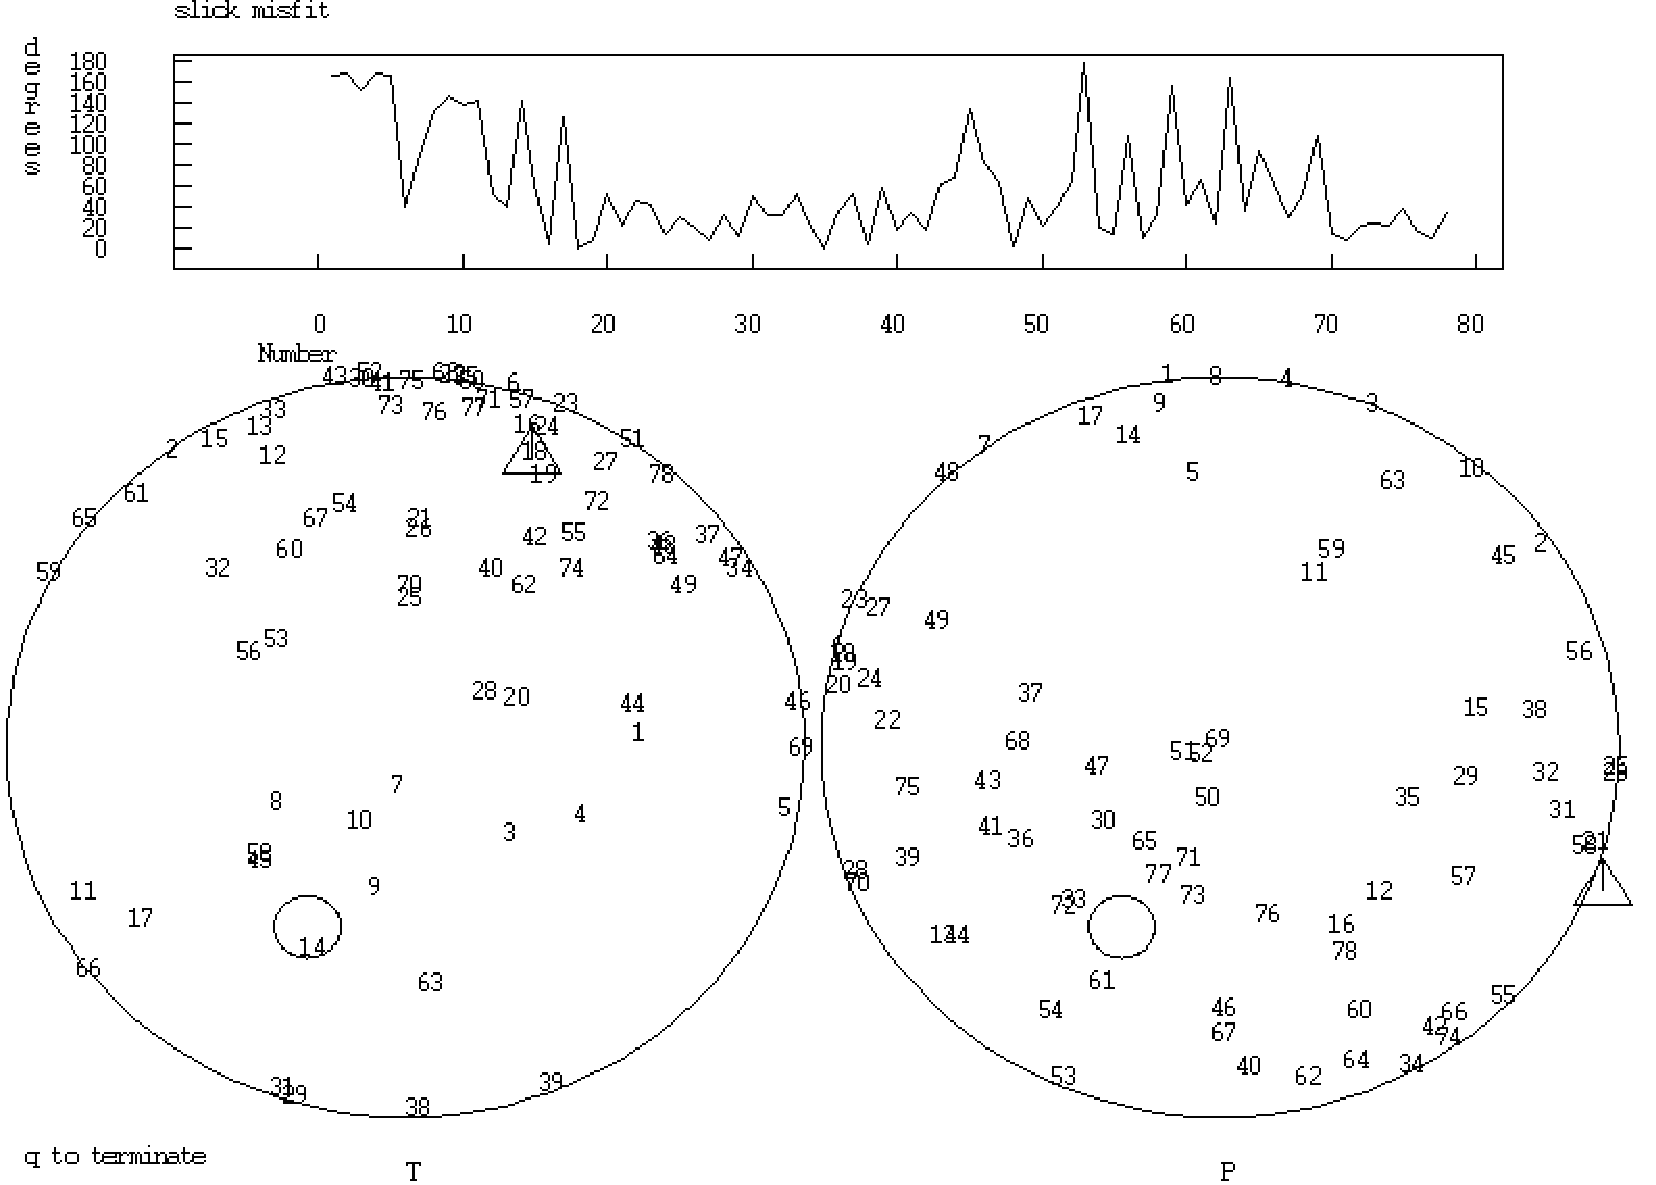
\includegraphics[width=0.9\linewidth]{fig/fps-slick}}
\caption{Left: The position of the T-axis given by the event numbers. The triangle is the SLICK minimum compressive stress direction and the circle is the null axis. Right: Corresponding for P-axis and the triangle is now the maximum compressive stress direction. Top: The misfit for each event as a function of event number. This figure can also show the cumulative misfit, see example run of FOC.}
\label{fig:fps-slick}
\end{figure}


Output files:\newline
Foc.out: P and T axis for all events, can be used as input to make rose diagrams.\newline
Foc\_events.out: The events used based on quality selection\newline
Foc\_pol.out: Statistics of polarities:

\begin{verbatim}
Stat     C    D
AZ05     3    2
MESC    18   60
VIF0     5    2
MIRA    10   32
VIF     44   19
LFA     52   18
PRCH    36    6
PVER    26    3
FRA0     0    2
AZ07     1    1
.
.
SET2     3    0
PSAN     1    3
 Sum of maximum number of polarities         570
 Sum of minimum number of polarities         158
\end{verbatim}

For each station the different polarities are counted and a sum of the consistent polarities are given at the end.
Foc.zmap: Input file in format used by ZMAP, notice direction of slip is used instead of strike of fault, see SLICK.\newline
Foc.slick and foc.slick.oput: See SLICK.

NOTE: FOC uses the first instance of the fault plane solution found in file for a particular event.

%}
